\documentclass[12pt]{article}
\usepackage{amsmath}
\usepackage{amssymb}
\usepackage{geometry}
\usepackage{enumerate}
\usepackage{natbib}
\usepackage{float}%稳定图片位置
\usepackage{graphicx}%画图
\usepackage[english]{babel}
\usepackage{a4wide}
\usepackage{indentfirst}%缩进
\usepackage{enumerate}%加序号
\usepackage{multirow}%合并行
\title{\large UM-SJTU JOINT INSTITUTE\\Intrapreneurship\\(VX423)\\\ \\\ \\\ \\\ \\\ \\\ \\\ \\\ \\\ \\\ \\\
Individual Report\\\ \\\ Intrapreneurship in SIIDI \\\ \\\ \\\ \\\ \\\ \\\ \\\ }
\author{Name: Pan Chongdan\\ID: 516370910121}
\date{Date: \today}

\begin{document}
\maketitle
\newpage
\section{Introduction of SIIDI}
SIIDI stands for Shanghai International Institute of Design and Innovation. The company was founded in 2017, aiming to do world-class practical research. The company mainly focuses on two areas, the first is sustainability research, including transportation ecosystem, urban quality living, high-tech big data service and Dutch Sustainability Day. The other area is Innovation service, including mental management, innovative thinking, leadership execution and field practice. 
\par SIIDI is a kind of consulting company which provides design and innovation service for start up companies and entrepreneurs. However, the biggest difference between SIIDI and other companies is that SIIDI focus more on making social welfare rather than making profit. Also, the strong connection between SIIDI, government and university is another feature of the institute. 
\section{Business Function of SIIDI}
\subsection{Marketing}
\par The main services provided by SIIDI is workshop and advice about design and innovation. The customers for the workshops are mainly workers from other companies, who want to gain some knowledge about design thinking. Other customers for SIIDI are start up companies or entrepreneurs who need SIIDI's help to incubate projects or make a model transformation. All of these services are at reasonable price. The workshops are always hold in the company or at public area, so it's a good way for the company to make promotion. Another promotion channel for the company is Internet and the company will publish an article on its official account after an activity is hold to increase its publicity. The main strategy for SIIDI is to use workshop's to attract customers and then work with them together to incubate innovative projects.
\subsection{Finance and Accounting}
\par SIIDI doesn't have a quite complicated finance and accounting including a lot loans because it's firstly founded by the government and 5 top universities in Shanghai. As a result, SIIDI is a company focusing more on making soical welfare than making profit. Actually, the company mainly get profits through making workshop and providing consulting service for cooperative enterprise.
\subsection{Human Resources}
\par SIIDI's human resources mainly include 3 parts:
\subsubsection{Universities}
Since SIIDI was firstly founded by 5 universities, there is a strong connection between the company and universities. Experts from universities will often come to SIIDI and give some advice for SIIDI's project.  For example, a professors from Tongji University once gave us a suggestion about how to solve the waste problem. The dean sets design thinking as the methodology of the institute's research. Also, interns from universities are also important resources for SIIDI, since they can provide more skills that SIIDI needs to realize their projects. SIIDI also uses this way to help interns to gain practical experience during their internship, which is a good way to help the education about entrepreneurship.
\subsubsection{Experts in Design Thinking}
Design thinking is the main culture in SIIDI, and a it's the basic principle for all workers to carry out their projects. Also SIIDI builds a relaxing environment with flat management, which means all of us do our job through design thinking process, including empathy, define, ideate, prototype and test. Our mentors pay a lot of emphasize on field practices because empathy requires field practices for us to put ourselves into customers' position to make design.
\subsubsection{Customers}
SIIDI's customers are also its resources because they're incubate a project together. Usually, they will give SIIDI their idea and the general orientation about the projects.
\begin{figure}[H]
\centering
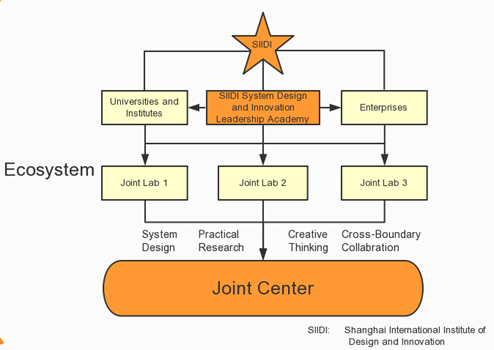
\includegraphics[scale=1]{p1.jpg}
\end{figure}
This is the big picture of SIIDI's business strategy. SIIDI mainly plays a role as intermediary in this cooperative corporate venturing between universities and companies and sets a joint labs to incubate projects together.
\section{Case Study: Waste Management Project}
The waste management project is the main project I participated in during my internship and the  following picture reflects how the company works. The project includes a smart bin which helps classification and monitors the classification status. The project also includes a GPS route planning system for garbage trucks.
\begin{figure}[H]
\centering
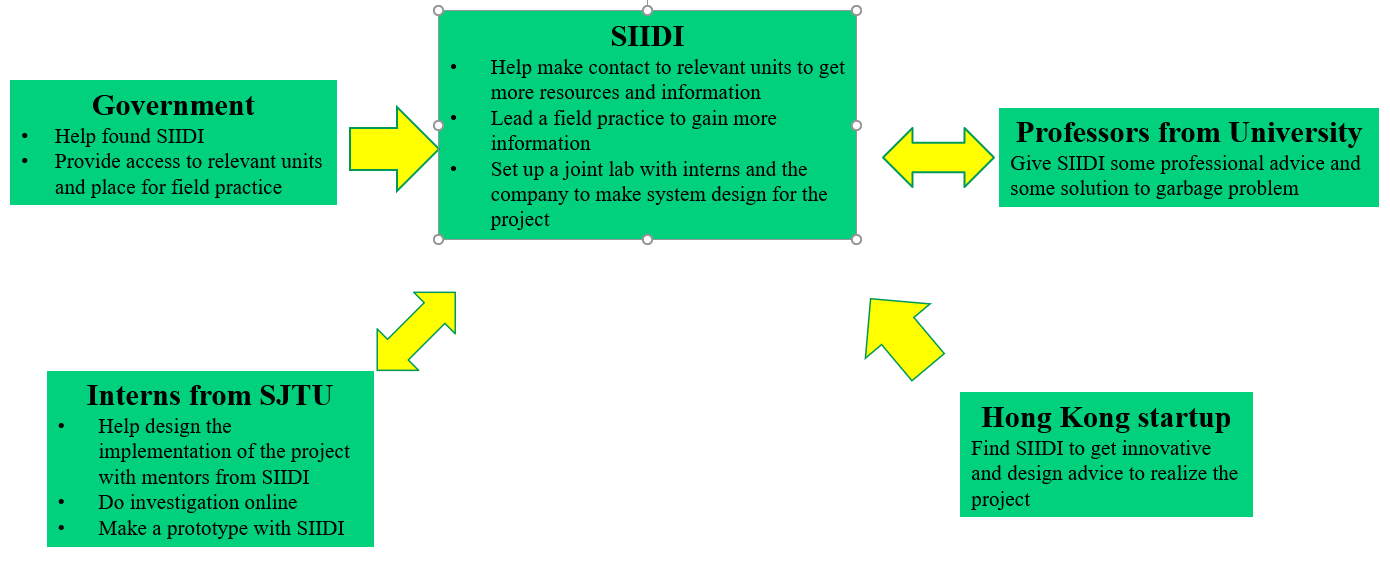
\includegraphics[scale=0.4]{p2.jpg}
\end{figure}
\paragraph{SIIDI's process in this project}
\begin{enumerate}
\item A HK company found SIIDI through SIIDI's distribution channel, seeking for advice on how to incubate a waste management project
\item SIIDI made contact with university alliance and got some advice from experts on environmental management. SIIDI also make contact with the government to get access to relevant units for information on transportation about garbage.
\item SIIDI set a joint lab with the start company and interns to design the implementation of the project and studied how to make a prototype.
\item SIIDI will make contact with real estate to get an opportunity to make field practice and interview to make the products from the project convenient for people at all ages.
\end{enumerate}
\paragraph{My work in this project}
\begin{enumerate}
\item Be a volunteer in a workshop on design thinking hold by SIIDI in Dec. 2019 and get a general idea about the design thinking.
\item Got a rough idea about the waste management project and started to search for examples and information online on Feb.26th.
\item Read and analyzed some reading material from mentors to get a deeper understanding about design thinking process on Mar.3rd
\item Started to make the system design for the implementation of the project based on design thinking process from Mar.9th
\item Drew a concept picture for the smart bin and decided its main functions on Mar.27th.
\item Made investigation online to search best material and sensors for this project since Apr.3rd.
\item Started to build a prototype since Apr.10th
\end{enumerate}
\par This project reflects the opportunity for this company's entrepreneurship because such project must be carried out with support from government, which is the advantage of SIIDI. However, SIIDI are also taking some risking in doing this project because waste problem hasn't been solved for several years. When SIIDI came to university for advice, the experts suggested us give up the waste management idea. So this project is likely to fail and quite challenging for the company. However, I think the biggest motivation for SIIDI to put efforts in this project is that the project is environment and social friendly. If it succeeds, it will help the government a lot by creating much social welfare. From this project we can see the strong connection between government and SIIDI. The partnership with government also give SIIDI a better environment to carry out projects as well as ask the company to do some difficult projects. 
\section{Problem Analysis and Process Innovation}
During my internship for this project, some problems are reflected and I think SIIDI can solve it by doing some incremental process innovation within the company.
\subsection{Unclear Company Orientation}
Even though SIIDI is a kind of consulting company, its business orientation is not very clear in this project because we're asked to make a prototype for our customers, which needs a lot of engineering skills and experience. However, our mentor is specialized in marketing and designing so we are facing a lot of difficulties during this stage. In my opinion, after our designing process, we should send our blueprint to some manufacturers and ask them to make the prototype. If we finish the technology part of the project for our customers, I think SIIDI is more like a technology company, which is not it's main business and strong point. It's better for SIIDI to renewal its strategy in this project and bring in manufacturers or developers to this project, which can help speed up the development of prototype.
\begin{figure}[H]
\centering
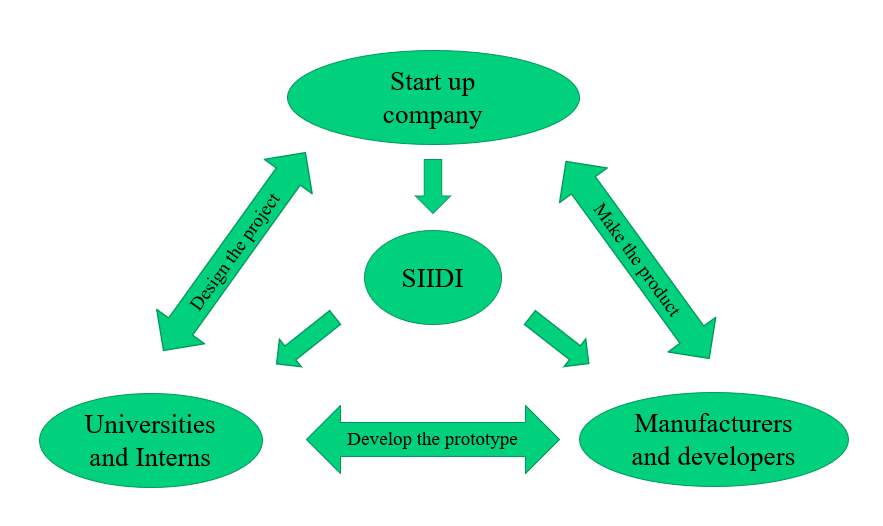
\includegraphics[scale=0.7]{p3.jpg}
\end{figure}
With help from new partners, SIIDI can focus on playing a role as a business incubator, which is specialized in providing service, mentoring and networking for its partners. 
\subsection{Lack of Schedule and Efficient Meeting}
SIIDI's flat manag increases the difficulty to coordinate everyone's time since everyone has his own project. As far as I know, this project was launched in July, 2018, but the pace is slow because no prototype has come out. In addition, the meetings are not very efficient. Once my colleague took a meeting until 7 pm and after the meeting he still didn't know what's the plan next week. Also, our partner wanted to have face to face with us meeting last week, but I still haven't met him. The main reason for the inefficiency is lack of schedule and consistency.
\begin{figure}[H]
\centering
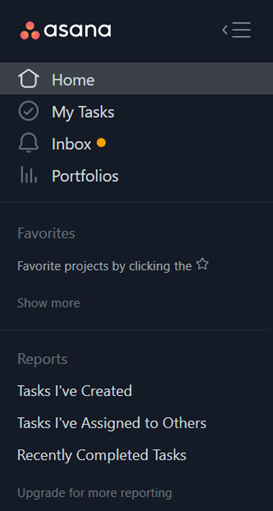
\includegraphics[scale=0.7]{p4.jpg}
\end{figure}
\par 
I think online project management software can be added into the company's management process because it can help team members to update his progress and draw the timeline, then the project's efficiency can be improved a lot. For example, this is an interface for Asana, a project management software developed by facebook. With help from Asana, project leader can assign tasks for its team members and set the due date or timeline. Partners of this project can update their progress and upload relevant files at any momonet. The application of online management software is an incremental innovation for the company's management and it can greatly improve the efficiency of the communication and sharing of a project.
\section{Business Environment and Competitors}
SIIDI has a unique business market due to strong connection with government because it's easier for SIIDI to get access which other consulting company can't have, like the government's resources management unit. It actually helps SIIDI reduce its competitors in market which requires a lot of information and partnership from government. 
\par However, consulting company which specializes in one field will be a strong competitor for SIIDI, because SIIDI provides design and innovation service in a broad area and it can't focus on one aspect of its domain. In addition, since SIIDI doesn't focus on making profit like other consulting company, it's not so aggressive in its market, which may slow the pace of the company's innovation. When our team are making design for the waste management project, we have also done some research for other project, including light system. As a result, SIIDI's efforts are spread over many projects, which is a possible reason why the project proceeds so slowly. 
\section{Domain Redefinition and Strategic Renewal}
Since strong connection with government and universities give SIIDI an advantage which its competitors can't have, SIIDI can play a role like an intermediary in projects, more than providing consulting service. The company can redefine its consulting domain by bringing more cooperative partners for its customers and help them get more information and resources. It's also a good way to help SIIDI broaden its consulting company because its prestige will be raised by contacting more partners.
\par As far as I know, SIIDI only works with its customers for one project while SIIDI's design thinking  can be applied for all areas. So SIIDI can renewal its strategy by providing a long time service based on design thinking. For example, after SIIDI help incubate a project with a company, it can keep helping the company transform its business model and broaden its market.
\section{Bibliography and Reference}
\begin{enumerate}
\item http://www.siidi.cn/
\item {https://app.asana.com/}
\end{enumerate}
\end{document}